\newchap{The $|V_{cb}|$ CKM element}\label{sec:vcb}
\vspace{-1cm}
\minitoc
This work aims to access the $|V_{cb}|$ element through the direct decay of a \PW boson at $\sqrt{s}=13 TeV$ with the recorded luminosity of the RunII.
\vspace{-0.25cm}
\section{The $V_{cb}$ element}\label{sec:vcb}
\begin{minipage}{\linewidth}
    \begin{minipage}{0.43\linewidth}
        The $V_{cb}$ element plays an important role in the unitarity of the CKM matrix. The radius of the unitarity-clock, the green circle centered in the origin in \Fig{fig:triangle}, is proportional to the ratio $|V_{ub}/V_{cb}|$, so $V_{cb}$ normalize the whole triangle \cite{Ricciardi2019DeterminationV_cb}.\\
        \\
        $|V_{cb}|$ is measured from the semileptonic inclusive and exclusive $b \to c\ell\nu$
        decays but the parton level amplitude, which is proportional to $|V_{cb}|^2$, has to be corrected by introducing form factors to consider the contributions by strong interactions in the meson. 
    \end{minipage}
    \hfill
    \begin{minipage}{0.55\linewidth}
        \vspace{-2.1cm}
        \begin{figure}[H]
            \centering
            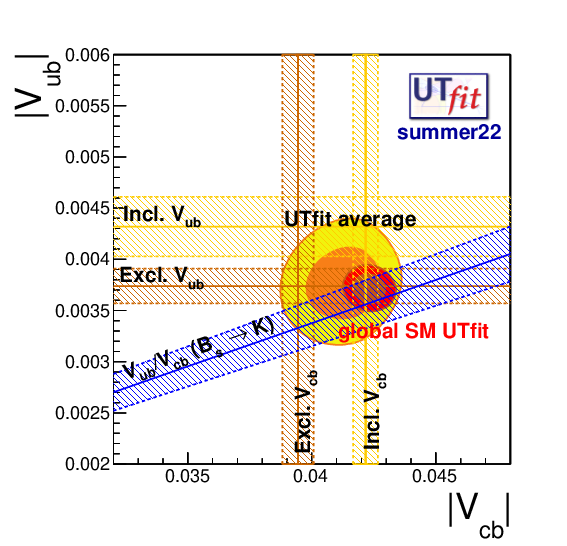
\includegraphics[width=\linewidth]{fig//chap02-theory/vubvcb.png}
            \caption{$|V_{cb}|$ and $|V_{ub}|$ global fit and averages of inclusive and exclusive measurements performed by the UTfit collaboration \cite{Bona2023NewScheme}}
            \label{fig:vcbvub}
        \end{figure}
    \end{minipage}
\end{minipage}\\
\\
These corrections inevitably lead to theoretical uncertainties that are of the same order as the experimental systematic uncertainties.\\
These issues also concern the $|V_{ub}|$ measurements.\\
A summary of the single measurements of the $|V_{cb}|$ element can be found in \cite{PDG_2022}.
\subsection{$|V_{cb}|$ from semileptonic B meson decays}
\paragraph*{Inclusive measurement}
The inclusive channel $B\to X_c \ell \nu$ is less model dependent than the exclusive one \cite{Smith2005DeterminationSpectra}.
The QCD contributions can be included by adding two terms in the amplitude: a perturbative term and a non-perturbative term.
\begin{equation}
    \Gamma(B\rightarrow X_c\ell\nu)=\frac{G_{F}^{2}m_{b}^{5}|V_{c b}|^{2}}{192\pi^{3}}[1+P(\alpha_{s},\mu,m_{b}/m_{c})+N(m_b,m_c,\mu_\pi^2,\mu_G^2,\rho_D^2,\rho_{LS}^3)]
\end{equation}
The QCD corrections are computed using the so-called Operator Product Expansion (OPE). OPE allows us to express the widths and moments of the kinematic distributions as a double expansion in $\alpha_S$ and $\Lambda_{QCD}/m_b$. These corrections are actually known up to the third order in $\Lambda_{QCD}/m_b$ \cite{Alberti2016TheVcb}.\\
This expansion depends on other parameters defined in the framework of the heavy quark effective field theory (HQET) that can be constrained through the study of other observables like the lepton energy, the transferred momentum or the hadronic mass \cite{Smith2005DeterminationSpectra} so the final fit has to be performed on an order of $\mathcal{O}(100)$ of observables.\\
The uncertainties of the inclusive measurements of $|V_{cb}|$ are  $\simeq 2\%$, mainly driven by theoretical uncertainties related to the determination of the HQET parameters \cite{Alberti2016TheVcb}.\\
The average of the inclusive measurements is \cite{Bordone2021ThreeVcb}
\begin{equation}
    |V_{cb}|\times10^3\text{ (incl)}=42.16\pm 0.50
\end{equation}

\paragraph*{Exclusive measurement}
The two main exclusive channels studied for $|V_{cb}|$ determination are the $\PAB \to D^* \ell \PAGnl$ and the $\PAB \to D \ell \PAGnl$.
The first channel was measured with an uncertainty of $\simeq 2\%$ with comparable contributions from theory and experiment, while the latter was measured with an uncertainty of the $\simeq 3\%$ but recently
some questions about the form factor parametrization were raised.\\
The exclusive measurement requires knowing six form factors that can be computed using lattice QCD (LQCD) techniques. In the limit of heavy quarks, the six form factors collapse into a single one, and corrections to the $m_b \to \infty$ limit can be obtained through the HQET framework \cite{PDG_2022}.\\
The average of the exclusive measurements is \cite{Bona2023NewScheme}
\begin{equation}
    |V_{cb}|\times10^3\text{ (excl)}=39.44\pm 0.63
\end{equation}

\paragraph*{The $|V_{cb}|$ puzzle}
The inclusive and exclusive measurements of the $V_{cb}$ element have always been incompatible as shown in \Fig{fig:vcbvub}.\\
Recently, a revision of the techniques involved in the calculations of the QCD contributions has narrowed the gap, but the $V_{cb}$ puzzle is still unresolved \cite{Bona2023NewScheme}: indeed the current determinations show a 7\% difference from each other.\\ 
Combining the measurements with a $\chi^2$ fit, the best-fit value is $|V_{cb}|_{\text{best}}=41.10$ that leads to a chi-square of $\chi^2=11.35$, corresponding to a p-value $p=7.2 \cdot 10^{-4}$, \ie to a tension of $\sim 3.3\sigma$.\\
\\
The determination of $|V_{cb}|$ through direct \PW decays would allow us to provide a new determination of $|V_{cb}|$ at a new energy scale ($\sqrt{s}=m_{\PW}$), avoiding complications and theoretical uncertainties due to non-perturbative QCD, tackling the $|V_{cb}|$ puzzle with a novel strategy.
\section{CKM measurements from hadronic W decays}
\subsection{LEP2 measurements}
The Large Electron-positron Collider (LEP) was an electron-positron collider that reached a peak energy in the center of mass of 209 GeV. It was built at CERN and is located in the tunnel that now hosts the LHC accelerator facility and started its physics program in 1989.\\
\\
The LEP2 physics program started in 1996, running at a center of mass energy  that was increased from 161\GeV to 209\GeV at the end of 1999, above the production threshold of WW pairs. 
In this period, each of the four LEP experiments, ALEPH, DELPHI, L3, and OPAL have collected  $\sim700 \text{pb}^{-1}$ of data above the WW pair production threshold, corresponding to over 10000 WW events per experiment \cite{Lu2008WLEP}.\\
\\
In this period, $\sim 10$ $\PW \to cb$ events per experiment were produced, making it impossible to provide a direct determination of $|V_{cb}|$ from inclusive \PW decays.\\
However, with more than 13000 hadronic W decays per experiment, the LEP experiments were able to access other elements in the charm sector of the CKM matrix.


\paragraph*{Rate of charm production}
ALEPH and OPAL performed a measure of the rate or $W\to cX$ decays on both semileptonic and fully hadronic WW pairs.
\begin{equation}
    R_c^W=\frac{\Gamma(W\to cX)}{\Gamma(W\to q\bar{q})}=\frac{|V_{cd}|^2+|V_{cs}|^2+|V_{cb}|^2}{|V_{cd}|^2+|V_{cs}|^2+|V_{cb}|^2+|V_{ud}|^2+|V_{us}|^2+|V_{ub}|^2}
\end{equation}
This is a unitarity test of the second row of the CKM matrix, indeed, if the unitarity hypothesis holds, it has to be $R_c^W=0.5$.
\\
\\
ALEPH performed the measurement extracting $R_c^W$ with a binned maximum-likelihood fit on the shape of the most c-tagged jet\cite{Barate1999ATag}.\\
The charm jet tagger was a feed-forward neural network with 12 variables as input that uses mainly information from charm lifetime, jet-shape properties, reconstruction of D mesons, and lepton identification.\\
\\
On the other hand, OPAL used a relative likelihood discriminant calculated for each jet to separate jets originating from charm quarks and jets from light quarks. This discriminant relies on jet and event shape properties, lifetime information, and lepton identification \cite{Abbiendi2000ADecays}.
\\
\\
The results of both experiments are consistent with the unitarity hypothesis with an uncertainty of $\sim 10\%$
\begin{equation}
\begin{aligned}
    R_c^W&=0.51 \pm 0.05 \text{ (stat)} \pm 0.03 \text{ (syst)} & \text{(ALEPH \cite{Barate1999ATag})}\\
    R_c^W&=0.481 \pm 0.042 \text{ (stat)} \pm 0.032 \text{ (syst)} & \text{(OPAL \cite{Abbiendi2000ADecays})}
\end{aligned}
\end{equation}\vspace{-0.001cm}
$R_C^W$ allow also an indirect measure of $|V_{cs}|$, subtracting the other $|V_{cx}|$ CKM elements in quadrature from $R_C^W$ obtained from other determinations.
\begin{equation}
\begin{aligned}
    |V_{cs}|&=1.00\pm0.11  \text{ (stat)} \pm 0.07 \text{ (syst)} & \text{(ALEPH \cite{Barate1999ATag})}\\
    |V_{cs}|&=0.969\pm0.058 & \text{(OPAL \cite{Abbiendi2000ADecays})}
\end{aligned}
\end{equation}
\begin{figure}[H]
    \begin{subfigure}{0.48\linewidth}
        \centering
         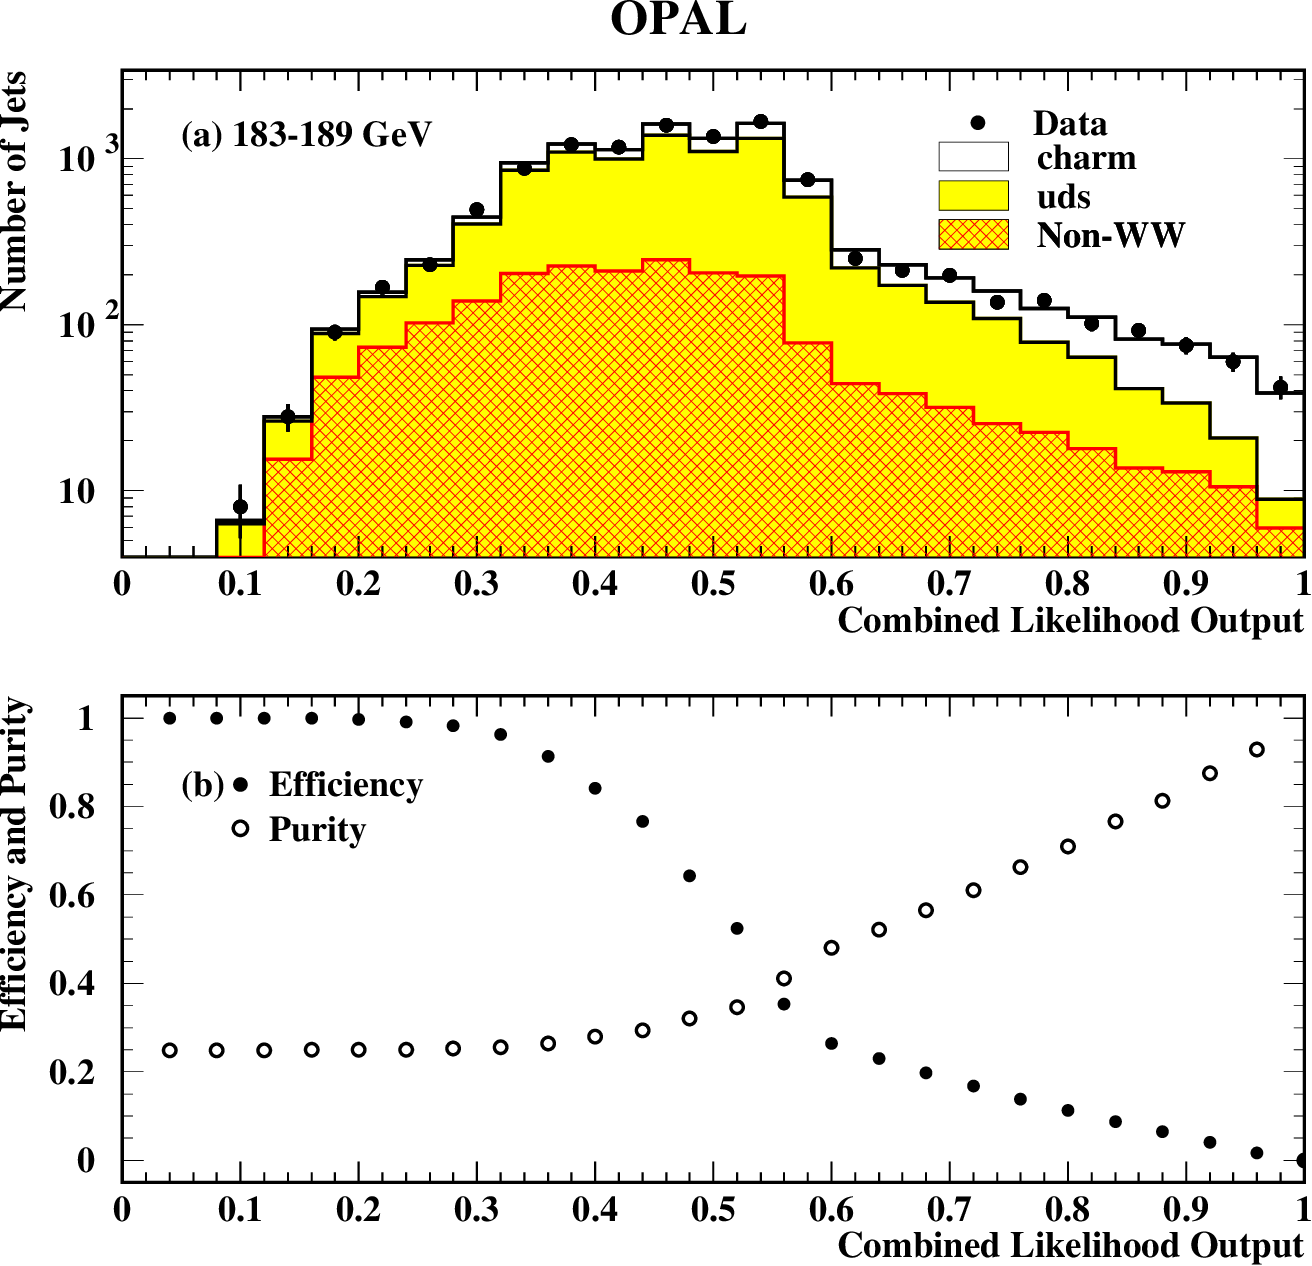
\includegraphics[width=\linewidth]{fig//chap02-theory/opal.png}
         \caption{OPAL: Output of the combined likelihood used to tag charm hadrons at 183–189 \GeV\cite{Abbiendi2000ADecays}.\\}
    \end{subfigure}
     \hfill
     \begin{subfigure}{0.475\linewidth}
         \centering
        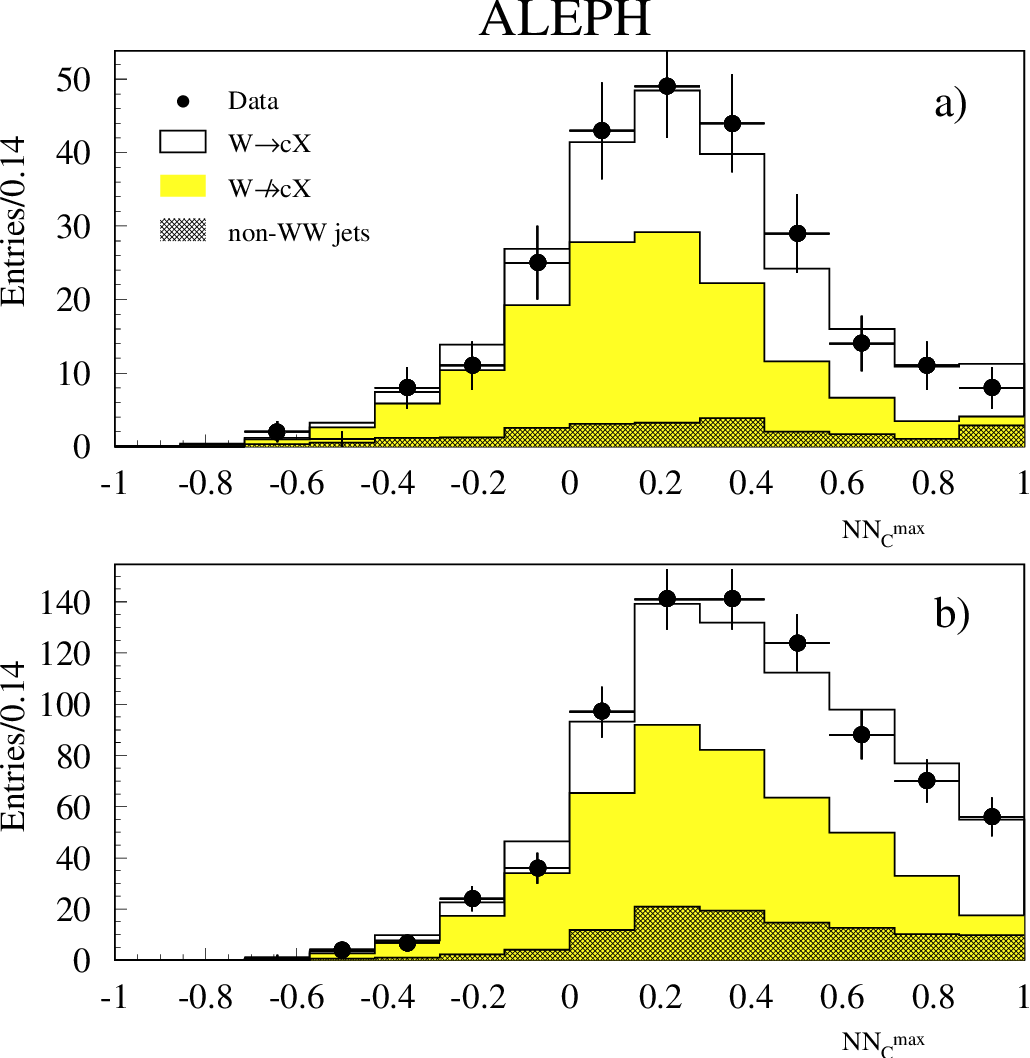
\includegraphics[width=\linewidth]{fig//chap02-theory/aleph.png}
         \caption{ALEPH: Maximum c tagging NN score for the dijet pairs. In the top panel there are the semileptonic WW pairs, in the bottom panel there are the fully hadronic \cite{Barate1999ATag}.}
     \end{subfigure}
        \label{fig:rc_lep}
\end{figure}
\vspace{-0.85cm}
\paragraph*{Direct measure of $|V_{cs}|$}
The $V_{cs}$ CKM element was measured directly from W decays by the DELPHI collaboration, using semileptonic and fully hadronic decays of WW pairs measuring $r^{(cs)}$ \cite{Abreu1998MeasurementLEP2}.
\vspace{-0.5cm}
\begin{equation}
    r^{(cs)}=\frac{\Gamma(W\to cs)}{\Gamma(W\to q\bar{q})}=\frac{|V_{cs}|^2}{2}
\end{equation}
where, in the last step, the unitarity of the CKM matrix is assumed.\\
To discriminate the signal, DELPHI built a cs tagger $P_{cs}$ that relies on information from the vertex and tracking detectors and on particle identification through RICH detectors.\\
\begin{minipage}{\linewidth}
\begin{minipage}{0.4\linewidth}
    \vspace{-1cm}
    The value of $V_{cs}$ was extracted fitting the $P_{cs}$ distribution of selected di-jet combinations by using the maximum likelihood method on a multinomial likelihood.
    \\
    The direct determination of $|V_{cs}|$ was performed on just 100 WW pairs collected in 1996, leading to a large statistical uncertainty of $\sim 30\%$\\
\end{minipage}
\hfill
\begin{minipage}{0.58\linewidth}
    \begin{figure}[H]
        \centering
        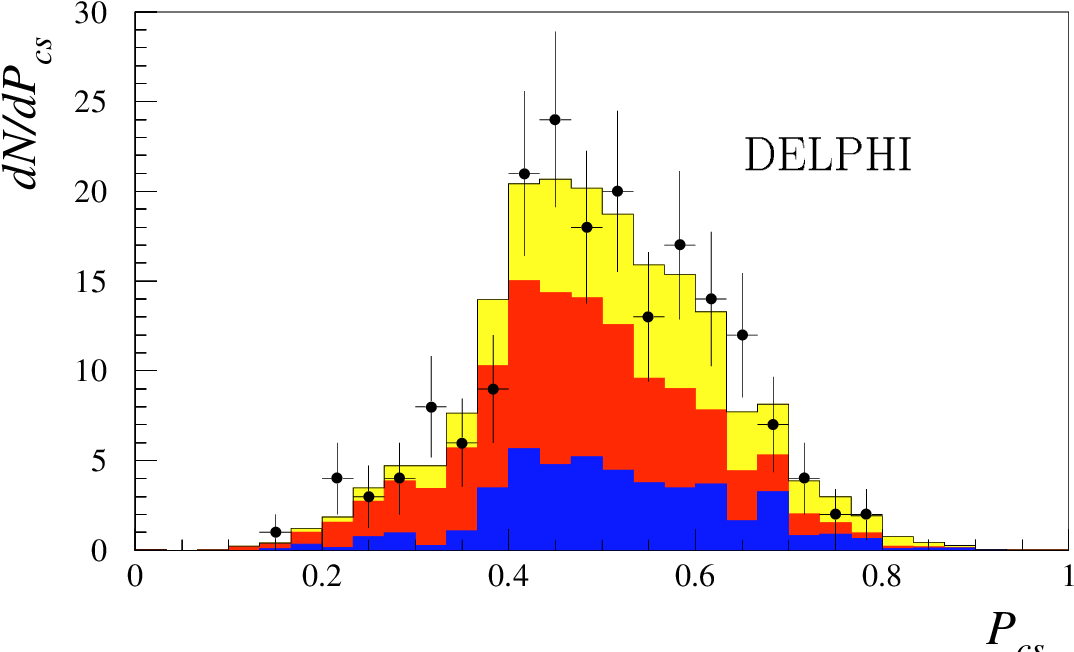
\includegraphics[width=\linewidth]{fig//chap02-theory/delphi.png}
        \caption{$P_{cs}$ distribution. The yellow is $W\to cX$ process, the red $W\to uX$, and the blue is the background \cite{Abreu1998MeasurementLEP2}.}
        \label{fig:enter-label}
    \end{figure}
\end{minipage}
\end{minipage}
\\
However, for the first time, DELPHI was able to provide a direct determination of $|V_{cs}|$ dominated by the statistical uncertainties and not dependent on theoretical systematics.
\begin{equation}
\begin{aligned}
    |V_{cs}|&=0.94^{+0.32}_{-0.26}  \text{ (stat)} \pm 0.13 \text{ (syst)} & \text{(DELPHI \cite{Abreu1998MeasurementLEP2})}
\end{aligned}
\end{equation}


\subsection{$|V_{cb}|$ with LHC data}
At LHC, in all the RunII, more than 26 billion single W bosons were produced: of these, more than 17 billion W bosons decay hadronically, which means that more than 14 million cb quark pairs can be obtained from the inclusive decay of \PW bosons.\\
Despite that, contrary to any electron-positron collider, an inclusive measurement of $\PW \to cb$ at a hadron collider would be an impossible task due to the large QCD background.\\
\\
To avoid it, it is possible to exploit the semileptonic decay of WW pairs and use the lepton to trigger the event and the hadronic \PW decay to measure the $\PW \to cb$ branching fraction.\\
As lepton $\ell$, we will only consider muons and electrons, due to the lower reconstruction efficiency of $\tau$s, that decay hadronically in the $64.8\%$ of cases.
\\
\\
The value of $|V_{cb}|$ can be extracted from the ratio of branching fractions in which the hadronic \PW decays into c and b quarks over the  \PW hadronic branching fraction
\begin{equation}
\begin{gathered}
    R_{cb}=\frac{\Gamma\left(\PW\PW \to \ell \nu\; cb\right)}{\Gamma\left(\PW\PW \to \ell \nu\; q\bar{q}\right)}=\\ =\frac{|V_{cb}|^2}{|V_{ud}|^2+|V_{us}|^2+|V_{ub}|^2+|V_{cd}|^2+|V_{cs}|^2+|V_{cb}|^2}
\end{gathered}
\end{equation}
and if we assume the unitarity of the CKM matrix
\begin{equation}
    R_{cb}=\frac{|V_{cb}|^2}{2}
\end{equation}

This kind of measure will be limited mainly by the b and c tagging systematic uncertainties, but the ratio of branching fractions should allow some cancellations.
\paragraph*{WW production}
At an energy of the center of mass of $\sqrt{s}=13 \TeV$, the direct WW production cross section is $\sigma_{pp\to\PW\PW}\sim118 \text{pb}$, which means that in all the RunII, more than 16 million of WW pairs were produced directly.\\
However, at LHC, the production cross-section of $\ttbar$ pairs is $\sim 7$ times greater than the direct WW production cross-section with $\sigma_{pp\to \ttbar}\sim832\text{pb}$ and, since the top quark decays in one b quark plus a \PW boson, we can exploit di-top decays as a \PW\PW factory.
\newpage
\paragraph*{Decay of WW pairs}\hspace{0.1cm}\\
\begin{minipage}{\linewidth}
    \vspace{0.5cm}
    \begin{minipage}{0.42\linewidth}
        \raggedright
            \centering
            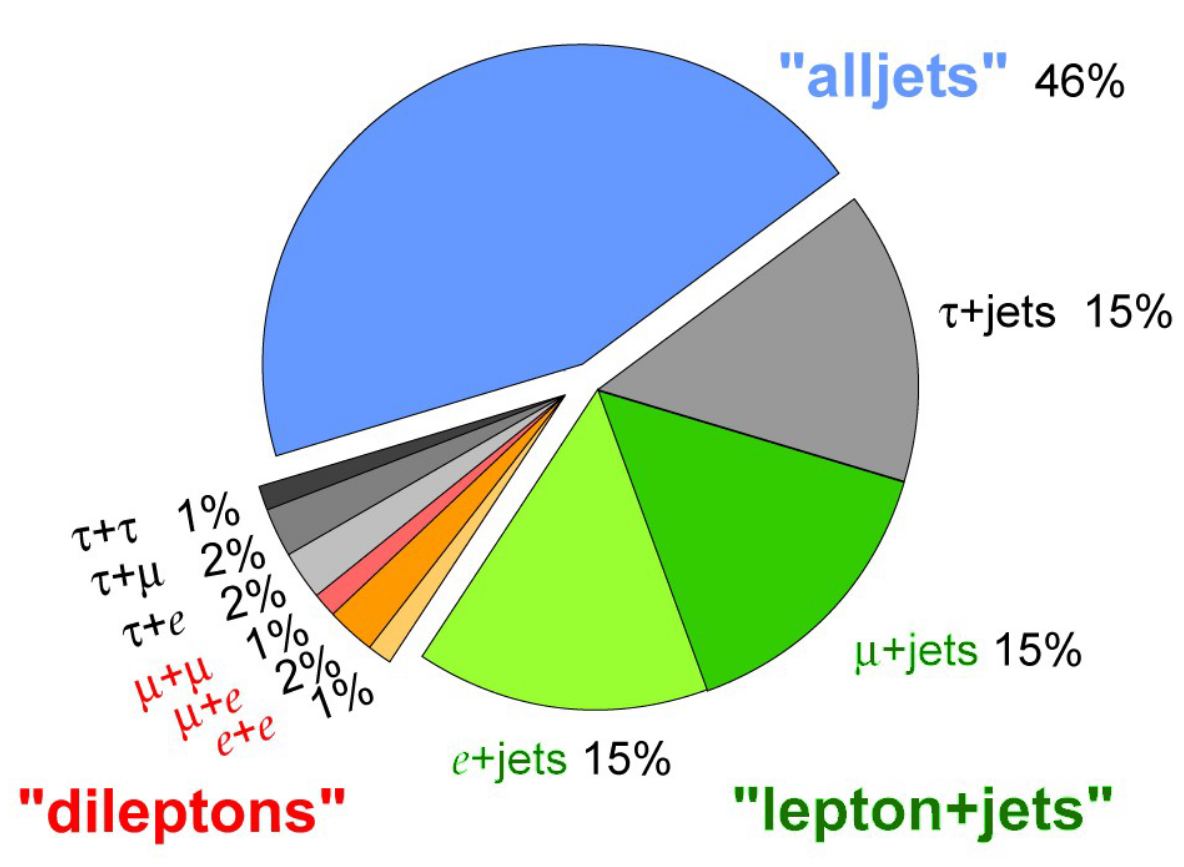
\includegraphics[width=\linewidth]{fig//chap02-theory/ttbr.png}
            \captionof{figure}{\PW pair decay branching fractions}
            \label{fig:ttbr}
    \end{minipage}
    \hfill
    \begin{minipage}{0.56\linewidth}
        \vspace{-1.1cm}
        \raggedright
        Since the branching fraction of the W decay are:
        \begin{itemize}
            \item 32.6\% \textbf{Hadronic} $\PW \to q\bar{q}$
            \item 67.4\% \textbf{Leptonic} $\PW \to \ell\nu$
        \end{itemize}
        the branching fractions of the $\PW^+\PW^-$ decay are:
        \begin{itemize}
            \item 45.5\% \textbf{Fully hadronic} $\PW\PW \to q \bar{q} q \bar{q}$. 
            \item 43.9\% \textbf{Semi leptonic} $\PW\PW \to q \bar{q} \ell \PGnl$
            \item 10.6\% \textbf{Di-leptonic} $\PW\PW \to \ell \PAGnl  \bar{\ell} \PGnl$
        \end{itemize}
        The branching ratio of the flavors of the $q_i\bar{q_j}$ pairs generated by \PW decays is given by the respective CKM elements $|V_{ij}|^2/2$.
    \end{minipage}

\end{minipage}
\\
\\
Since more than 110 million WW pairs were produced in the RunII through di-top decays, around 40000 $\PW \to cb$ events were produced in the $\ttbar$ semileptonic channel, while the amount of cb events produced by the semileptonic decay of directly produced WW pairs is around 6000.\\
\\
The amount of cb events provided by $\ttbar$ semileptonic decays in the RunII allows us to provide a new determination of $|V_{cb}|$ that, in case of a perfect selection, would reach the 0.5\% statistical precision, that is a huge improvement with respect the current 7\% difference between the current inclusive and exclusive determination obtained through the semileptonic decay of B mesons.\\
However, the separation between signal and background, which relies mainly on the b/c-tagging capabilities of the experiment, must be evaluated, along with the b/c-tagging systematic uncertainties.

\begin{table}[H]
    \centering
    \begin{tabular}{c|c|c|c|c}
        \toprule
        \multicolumn{5}{c}{$\PW \to cb$ events}\\
        \midrule
        \midrule
        \textbf{W} &  \multicolumn{2}{c|}{\textbf{WW}} & \multicolumn{2}{c}{$\bm{t\bar{t}}$} \\
        \midrule
          $1.4 \cdot 10^7$&  \multicolumn{2}{c|}{$1.8 \cdot 10^4$}  &  \multicolumn{2}{c}{$1.2 \cdot 10^5$} \\
        \midrule
        \textbf{Had} & \textbf{diHad} & \textbf{semiLept} & \textbf{diHad} & \textbf{semiLept}\\
        \midrule
         $1.4 \cdot 10^7$ & $1.2\cdot 10^4$ & $5.8 \cdot 10^3$ & $8.0 \cdot 10^4$ & $4.0\cdot 10^4$ \\
         \bottomrule

    \end{tabular}
    \caption{Amount of $\PW \to cb$ events produced per experiment in all the RunII at LHC for each process.}
    \label{tab:my_label}
\end{table}